\documentclass[12pt,a4paper]{article}

% ---------- Codificación e idioma ----------
\usepackage[utf8]{inputenc}
\usepackage[T1]{fontenc}
\usepackage[spanish,es-noshorthands]{babel}
\usepackage{lmodern}

% ---------- Paquetes útiles ----------
\usepackage[margin=2.5cm]{geometry}
\usepackage{graphicx}
\usepackage{xcolor}
\usepackage{booktabs}
\usepackage{array}
\usepackage{enumitem}
\usepackage{parskip}
\usepackage{verbatim}
\usepackage[hidelinks]{hyperref}
\usepackage{xurl}   % permite cortar las URLs largas para que no se salgan del margen

% ---------- Referencias con sangria francesa (APA) ----------
\newenvironment{referencias}
  {\begin{list}{}{%
     \setlength{\leftmargin}{1.6em}\setlength{\itemindent}{-1.6em}%
     \setlength{\labelwidth}{0pt}\setlength{\labelsep}{0pt}%
     \setlength{\itemsep}{0.7em}\setlength{\parsep}{0pt}}}
  {\end{list}}

% ---------- Colores ----------
\definecolor{azulUVG}{RGB}{30,90,150}
\definecolor{verde}{RGB}{46,139,87}
\definecolor{grisclaro}{RGB}{240,243,246}
\definecolor{gristexto}{RGB}{90,100,110}

% Secciones sin numerar para un estilo menos formal
\setcounter{secnumdepth}{0}
\pagestyle{plain}

\begin{document}

% =====================================================================
%  CARÁTULA
% =====================================================================
\begin{titlepage}
\begin{center}

\textbf{UNIVERSIDAD DEL VALLE DE GUATEMALA}\\
Facultad de Ingeniería\\[2cm]

\IfFileExists{logo uvg.png}{%
  
\includegraphics[width=0.35\textwidth]{logo uvg.png}\\[2.5cm]
}{%
  \vspace*{2.5cm}
}

{\LARGE\textbf{Caso de Estudio 2}}\\[0.6cm]
{\large Diagnóstico del sistema de puntos MiMcDonald's Guatemala}\\[1.5cm]

Diego Linares\\[0.2cm]
Andy Fuentes\\[0.2cm]
Christian Echeverria\\[0.2cm]
Diederich Solis\\[1cm]

Machine Learning Engineering\\[2cm]

Septiembre de 2026

\end{center}
\end{titlepage}

% ---------------------------------------------------
\section{Resumen de la situación}

McDonald's Guatemala, operado por la franquicia maestra \textbf{McDonald's Mesoamérica} (126
restaurantes), lanzó el 27 de agosto de 2025 su programa de lealtad \textbf{MiMcDonald's}, que
reemplazó a \emph{Puntos McDelivery}. Quienes diseñaron el sistema ya no están en la empresa y no
quedó documentación. Nos contrataron como consultores para diagnosticarlo y proponer mejoras en
una semana.

El cliente no nos entregó datos, así que el reto fue doble: entender el sistema desde afuera y
demostrar que lo entendimos. Lo trabajamos con \textbf{CRISP-DM}, fase por fase:

\begin{enumerate}[leftmargin=1.4em]
\item \textbf{Reconstruimos las reglas} del programa desde sus Términos y Condiciones oficiales:
22 reglas y 8 vacíos de documentación (McDonald's Guatemala, s.f.-a).
\item \textbf{Inferimos la arquitectura de datos actual} y la dibujamos.
\item Construimos una \textbf{réplica en miniatura} con arquitectura \textbf{medallion} (Bronze,
Silver y Gold) en Databricks Free Edition, alimentada con \textbf{datos sintéticos} que respetan
las reglas y traen 18 tipos de error inyectados a propósito.
\item Hicimos una \textbf{prueba funcional (POC)}: \textbf{39 de 39 pruebas OK}. El pipeline
calcula los saldos de 5,150 clientes sin una sola diferencia contra una contabilidad
independiente.
\item Integramos un \textbf{modelo de ML}: un recomendador de recompensas que acierta lo que el
cliente canjea un 39\,\% más que recomendar lo más popular.
\end{enumerate}

\textbf{Hallazgos principales:}

\begin{center}
\renewcommand{\arraystretch}{1.4}
\begin{tabular}{|>{\raggedright\arraybackslash}p{7.2cm}|>{\raggedright\arraybackslash}p{6.4cm}|}
\hline
\textbf{Hallazgo} & \textbf{Evidencia} \\
\hline
El tope de 1,000 puntos diarios castiga a McDelivery, el canal que más gasta & Pierde el 39\,\%
de sus puntos, contra un 17\,\% en caja \\
\hline
Breakage alto: muchos puntos vencen sin usarse & 8.1 millones de puntos vencidos, el 44\,\% de lo
acumulado por compras \\
\hline
La app no valida el mínimo de canje en McDelivery (Q50 / Q60) & 33 canjes por debajo del
mínimo \\
\hline
El catálogo no atiende a todos: desayuno y familias no tienen una recompensa accesible de su
gusto & El café, la única recompensa barata de desayuno, salió del catálogo en junio \\
\hline
No hay verificación de identidad & 150 cuentas duplicadas cobrando la bienvenida \\
\hline
No se publicó la tasa de conversión del programa anterior (1 pt/Q $\rightarrow$ 10 pts/Q) &
Riesgo reputacional y contable \\
\hline
\end{tabular}
\end{center}

% ---------------------------------------------------
\section{1. Cómo lo trabajamos}

\begin{center}
\renewcommand{\arraystretch}{1.4}
\begin{tabular}{|>{\raggedright\arraybackslash}p{3.8cm}|>{\raggedright\arraybackslash}p{4.6cm}|>{\raggedright\arraybackslash}p{5.2cm}|}
\hline
\textbf{Fase CRISP-DM} & \textbf{Pregunta} & \textbf{En el repositorio} \\
\hline
Entendimiento del negocio & ¿Qué reglas tiene el programa? & \texttt{docs/01} \\
\hline
Entendimiento de los datos & ¿Qué sistemas generan datos y con qué problemas? & \texttt{docs/02},
\texttt{diagramas/} \\
\hline
Preparación de datos & Réplica medallion & \texttt{notebooks/00} a \texttt{03} \\
\hline
Modelado & Recomendador de recompensas & \texttt{notebooks/04} \\
\hline
Evaluación & POC contra la hoja de respuestas & \texttt{notebooks/05} \\
\hline
Despliegue & Recomendaciones y este reporte & \texttt{reporte/} \\
\hline
\end{tabular}
\end{center}

\textbf{Herramientas:} Databricks Free Edition (Serverless, Unity Catalog, Volumes, tablas Delta y
MLflow), PySpark, pandas, scikit-learn, Mermaid para los diagramas y GitHub conectado al workspace
con Git folders.

% ---------------------------------------------------
\section{2. Diagnóstico del sistema actual}

\subsection{Las reglas que reconstruimos}

\begin{center}
\renewcommand{\arraystretch}{1.35}
\begin{tabular}{|>{\raggedright\arraybackslash}p{1.6cm}|>{\raggedright\arraybackslash}p{3.8cm}|>{\raggedright\arraybackslash}p{8.2cm}|}
\hline
\textbf{ID} & \textbf{Regla} & \textbf{Valor} \\
\hline
R1--R2 & Acumulación & 10 puntos por cada Q1, redondeando hacia arriba (precios con IVA) \\
\hline
R4--R5 & No acumulan & Donaciones y productos canjeados \\
\hline
R6--R7 & Canales & Acumulan: mostrador, AutoMac, kioscos, McCafé, Centros de Postre y la app.
\textbf{No} acumulan: apps de terceros, Call Center y WhatsApp \\
\hline
R8 & Tope de acumulación & 1,000 puntos por día \\
\hline
R9 & Acreditación & Máximo 24 horas, lo que indica procesamiento por lotes nocturno \\
\hline
R10--R11 & Vencimiento & 365 días por lote, con aviso 30 días antes \\
\hline
R12--R13 & Límites de canje & 15,000 puntos por día y 3 ofertas por pedido \\
\hline
R14 & Canje irreversible & Los puntos no se devuelven aunque se anule la orden \\
\hline
R15 & Mínimo para canjear en McDelivery & Q50 en desayuno y Q60 en almuerzo y cena \\
\hline
R16 & Catálogo & De 3,000 a 7,500 puntos; cambia sin previo aviso \\
\hline
R17 & Bienvenida & Quesoburguesa al registrarse y 1,000 puntos con la primera compra \\
\hline
R20 & Territorio & Solo Guatemala, aunque la plataforma se comparte con Honduras \\
\hline
R21 & Migración & Los puntos anteriores ``se convierten automáticamente'' \\
\hline
\end{tabular}
\end{center}

\subsection{Lo que la documentación no dice}

Un sistema que nadie documentó siempre tiene huecos. Los reportamos y, para poder avanzar, los
resolvimos con supuestos explícitos que el cliente debe validar:

\begin{center}
\renewcommand{\arraystretch}{1.35}
\begin{tabular}{|>{\raggedright\arraybackslash}p{1cm}|>{\raggedright\arraybackslash}p{7.2cm}|>{\raggedright\arraybackslash}p{5.4cm}|}
\hline
\textbf{ID} & \textbf{Vacío} & \textbf{Supuesto en la réplica} \\
\hline
H1 & No se publica la tasa de conversión del programa anterior & $\times$10 (conserva el valor en
quetzales) \\
\hline
H2 & No es explícito si el IVA suma puntos & Sí: se usa el total pagado \\
\hline
H3 & No se dice qué pasa con los puntos de una orden anulada & No acumulan \\
\hline
H4 & La acreditación en 24 h sugiere procesamiento batch & Pipeline diario \\
\hline
H5 & El tope diario no define zona horaria ni orden de corte & Día de Guatemala, en orden
cronológico \\
\hline
H6 & ``Dos correos = dos cuentas'' y el teléfono es opcional & Se detectan cuentas de la misma
persona \\
\hline
H7 & La recompensa más barata exige Q300 y al menos 3 días de compra & Se analiza en Gold \\
\hline
H8 & La nube del franquiciado no es pública; Google Cloud es del corporativo (McDonald's
Corporation, 2023) & Se reporta como supuesto \\
\hline
\end{tabular}
\end{center}

\subsection{Arquitectura de datos actual (inferida)}

Las compras en el restaurante pasan por el POS y llegan al motor de lealtad \textbf{por lotes};
las de la app entran directo. Un detalle importante: el POS solo conoce el código QR del
cliente, no quién es. Borde punteado significa inferido; en rojo, los canales que no acumulan.

\begin{center}
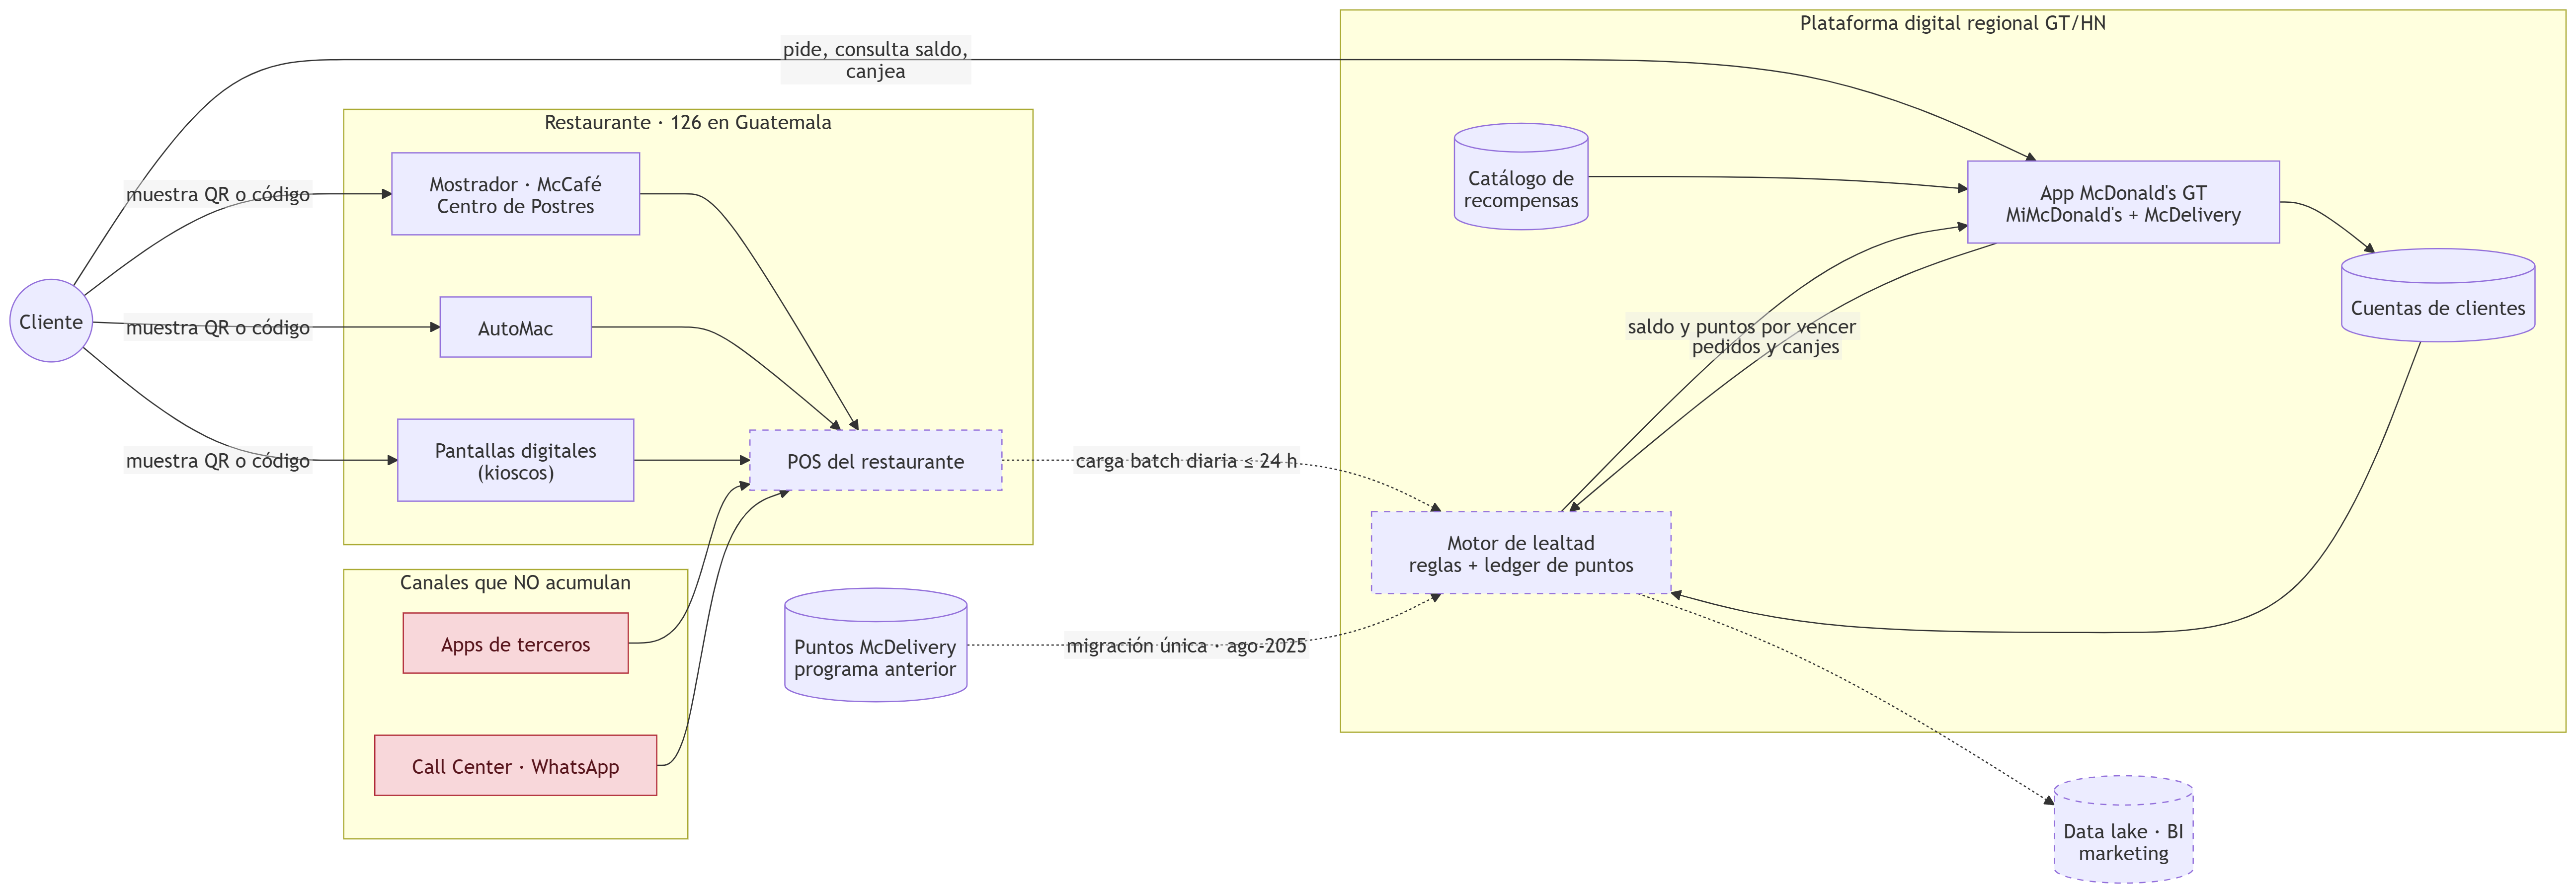
\includegraphics[width=\textwidth]{imagenes/arquitectura_actual.png}
\end{center}

% ---------------------------------------------------
\section{3. La réplica en miniatura}

\subsection{Datos sintéticos}

Como no teníamos datos, el notebook \texttt{00\_generador\_datos.py} simula los \textbf{6 sistemas
origen}, cada uno con su propio formato, igual que en la realidad: el POS manda CSV con hora
local, la app manda JSON anidado con hora UTC y campos en inglés, y el CRM manda un solo arreglo
JSON. Son 5,250 cuentas, 30 restaurantes y 13 meses de operación (56,239 tickets), con
\textbf{18 tipos de error} inyectados: archivos reenviados, canales mal escritos, precios con coma
decimal, códigos QR inexistentes, eventos duplicados, cuentas duplicadas, saldos negativos, entre
otros.

La decisión que más nos sirvió fue que el generador lleve \textbf{su propia contabilidad de
puntos} en Python puro y la guarde como \emph{hoja de respuestas} en un Volume aparte, que el
pipeline nunca lee. Así, al final, pudimos comparar dos implementaciones independientes de las
mismas reglas.

\subsection{Arquitectura medallion}

\begin{center}
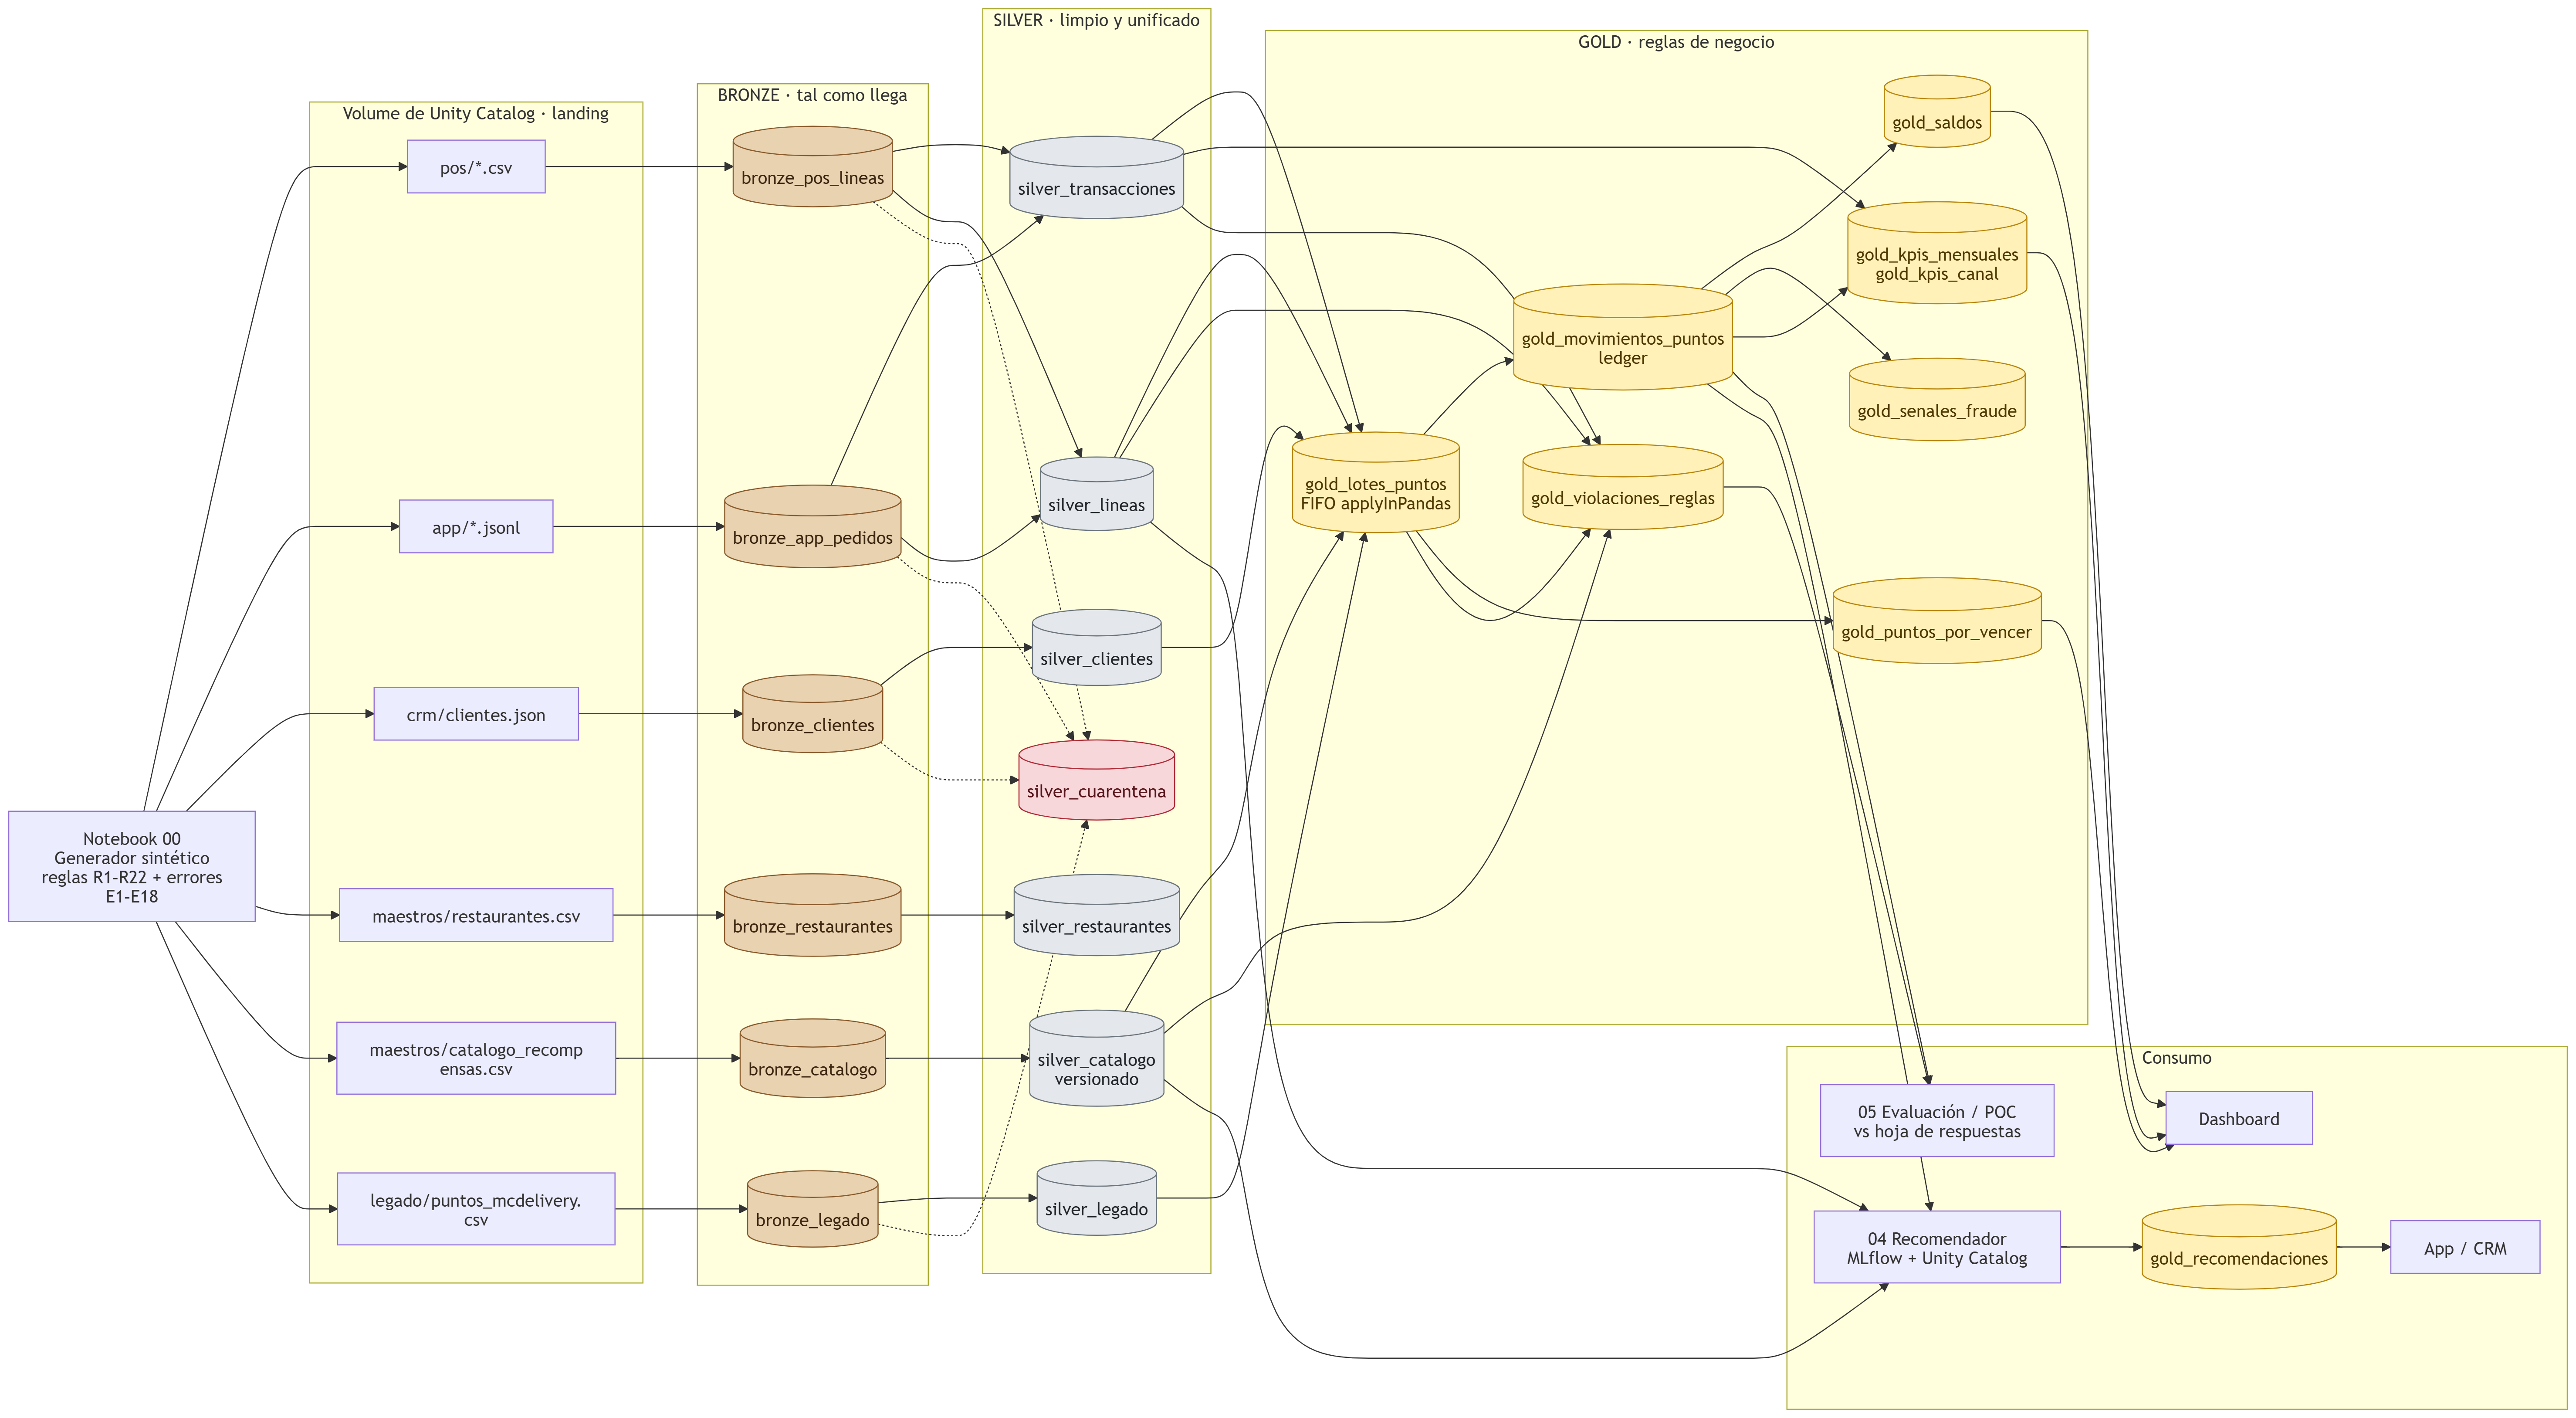
\includegraphics[width=\textwidth]{imagenes/arquitectura_replica.png}
\end{center}

\begin{center}
\renewcommand{\arraystretch}{1.4}
\begin{tabular}{|>{\raggedright\arraybackslash}p{2cm}|>{\raggedright\arraybackslash}p{8.6cm}|>{\raggedright\arraybackslash}p{3cm}|}
\hline
\textbf{Capa} & \textbf{Qué hace} & \textbf{Tablas} \\
\hline
Landing & Los archivos tal como los ``envían'' los sistemas & Volume \\
\hline
Bronze & Cada fuente como tabla, \textbf{sin corregir nada} (todo texto), más el archivo de origen y
la fecha de ingesta & 6 tablas \\
\hline
Silver & Limpia, tipa, deduplica y \textbf{unifica POS y app} en hora de Guatemala; lo
irrecuperable va a cuarentena con su motivo & 8 tablas \\
\hline
Gold & Aplica las \textbf{reglas del programa}: ledger de puntos, saldos, vencimientos, KPIs y
violaciones & 8 tablas \\
\hline
\end{tabular}
\end{center}

En nuestra opinión, lo más importante que aprendimos del medallion es la frontera entre capas:
\textbf{Silver describe qué pasó y Gold decide qué significa}. Si mañana McDonald's cambia la tasa
de puntos, solo se toca Gold. Y como los puntos vencen por lote, \textbf{el saldo nunca se guarda:
se calcula} sumando un libro de movimientos (\emph{ledger}), igual que en contabilidad. Así
cualquier saldo se puede auditar hasta la compra que lo originó.

% ---------------------------------------------------
\section{4. Prueba funcional (POC) del sistema de puntos}

\subsection{Procedimiento}

\begin{enumerate}[leftmargin=1.4em]
\item En Databricks: \textbf{Workspace $\rightarrow$ Create $\rightarrow$ Git folder} con la URL
del repositorio.
\item Correr en orden, en Serverless: \texttt{00\_generador\_datos}, \texttt{01\_bronze},
\texttt{02\_silver}, \texttt{03\_gold}, \texttt{04\_recomendador} y \texttt{05\_evaluacion}.
\item \texttt{05\_evaluacion} compara todo contra la hoja de respuestas y guarda el resultado en
la tabla \texttt{eval\_resultados\_poc}.
\end{enumerate}

\subsection{Código clave}

\textbf{El tope diario sin ciclos.} Si \texttt{S} es la suma acumulada de las compras del día,
cada compra recibe $\min(1000, S) - \min(1000, S - \mathrm{puntos})$, y eso cabe en una sola
\emph{window function}:

\begin{verbatim}
mismo_dia = (Window.partitionBy("customer_id", "fecha_gt")
                   .orderBy("fecha_hora_gt", "transaccion_id")
                   .rowsBetween(Window.unboundedPreceding,
                                Window.currentRow))
compras = (compras
    .withColumn("suma_dia", F.sum("puntos_calculados").over(mismo_dia))
    .withColumn("puntos_otorgados",
        F.least(tope, F.col("suma_dia"))
        - F.least(tope, F.col("suma_dia") - F.col("puntos_calculados"))))
\end{verbatim}

\textbf{Vencimiento por lotes (FIFO).} Esto no cabe en SQL: lo que vence de un lote depende de lo
que consumieron los canjes anteriores, y eso depende de lo que venció antes. Lo resolvimos cliente
por cliente con \texttt{applyInPandas}, que Spark reparte en paralelo:

\begin{verbatim}
def procesar_lotes(pdf):
    lotes = []                                    # [fecha, puntos_restantes]
    for fila in pdf.sort_values(["fecha_gt", "fecha_hora_gt"]).itertuples():
        vencer(fila.fecha_gt)                     # fecha del lote + 365 <= hoy
        if fila.puntos > 0:
            lotes.append([fila.fecha_gt, fila.puntos])   # abono: nace un lote
        else:
            costo = -fila.puntos                         # canje: lo mas viejo
            for lote in lotes:
                usar = min(lote[1], costo)
                lote[1] -= usar; costo -= usar

lotes = movimientos.groupBy("customer_id").applyInPandas(procesar_lotes, ...)
\end{verbatim}

\subsection{Resultados: 39 de 39 pruebas OK}

\begin{center}
\renewcommand{\arraystretch}{1.4}
\begin{tabular}{|>{\raggedright\arraybackslash}p{4.2cm}|>{\raggedright\arraybackslash}p{7.2cm}|p{1.6cm}|}
\hline
\textbf{Parte} & \textbf{Qué se probó} & \textbf{OK} \\
\hline
A. Reglas & Cada regla sobre \textbf{todos} sus casos reales, con el resultado esperado calculado
aparte & 12 / 12 \\
\hline
B. Calidad de datos & Los registros detectados contra los inyectados, uno por uno & 18 / 18 \\
\hline
C. Saldos & Gold contra la hoja de respuestas, cliente por cliente & 8 / 8 \\
\hline
D. Recomendador & Recomendaciones contra el gusto real de cada cliente & 1 / 1 \\
\hline
\end{tabular}
\end{center}

\textbf{Parte A, algunos ejemplos.} Q12.75 $\times$ 10 = 127.5 $\rightarrow$ \textbf{128} puntos
(R2). El cliente C002481 calculó 5,430 puntos en un día y recibió \textbf{1,000} (R8). De los
canjes de Big Tasty, 158 costaron 7,000 puntos y 87 costaron 7,500, según la fecha del canje
(R16). Hubo 1,378 tickets de Call Center, WhatsApp y apps de terceros con el cliente identificado,
y ninguno acumuló (R7).

\textbf{Parte B.} No quisimos comparar solo conteos, porque dos errores distintos podrían
compensarse. Comparamos los registros: para los 17 tipos de error, \textbf{0 faltantes y 0 falsas
alarmas}. Es la misma lógica de \emph{precision} y \emph{recall} de un clasificador, pero
aplicada a la limpieza de datos.

\textbf{Parte C.} Dos implementaciones escritas por separado (Python puro en el generador y Spark
en Gold) llegan al mismo resultado:

\begin{center}
\renewcommand{\arraystretch}{1.35}
\begin{tabular}{|p{5cm}|r|p{4.2cm}|}
\hline
\textbf{Métrica} & \textbf{Total} & \textbf{Clientes con diferencia} \\
\hline
Acumulados por compras & 18,581,394 & 0 de 5,150 \\
\hline
Bienvenida & 4,336,000 & 0 de 5,150 \\
\hline
Migrados del programa anterior & 17,835,600 & 0 de 5,150 \\
\hline
Canjeados & 20,729,000 & 0 de 5,150 \\
\hline
Vencidos & 8,097,012 & 0 de 5,150 \\
\hline
Perdidos por el tope diario & 5,277,554 & 0 de 5,150 \\
\hline
\textbf{Saldo al 20 de septiembre de 2026} & \textbf{11,926,982} & \textbf{0 de 5,150} \\
\hline
\end{tabular}
\end{center}

% ---------------------------------------------------
\section{5. Hallazgos del diagnóstico}

\subsection{El tope diario castiga a los pedidos grandes}

Con 10 puntos por quetzal y un tope de 1,000 puntos diarios, todo lo que se gaste arriba de Q100
en un día no genera puntos. En McDelivery el 67\,\% de los pedidos pasa de Q100, así que el canal
de los clientes que más gastan es el peor tratado:

\begin{center}
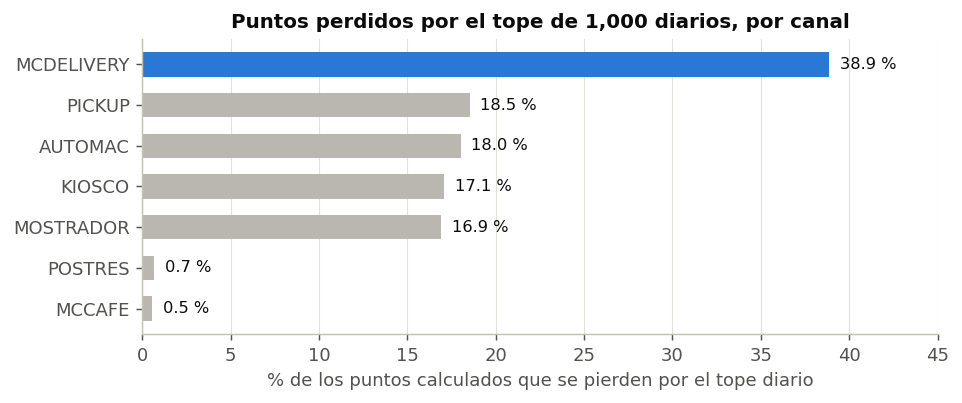
\includegraphics[width=0.85\textwidth]{imagenes/grafica_tope_canal.png}
\end{center}

\subsection{Los puntos migrados vencen en masa al año}

Los puntos del programa anterior se abonaron en agosto y septiembre de 2025, y vencen todos juntos
un año después. Para la empresa es un pasivo que desaparece; para los clientes más antiguos, una
mala experiencia:

\begin{center}
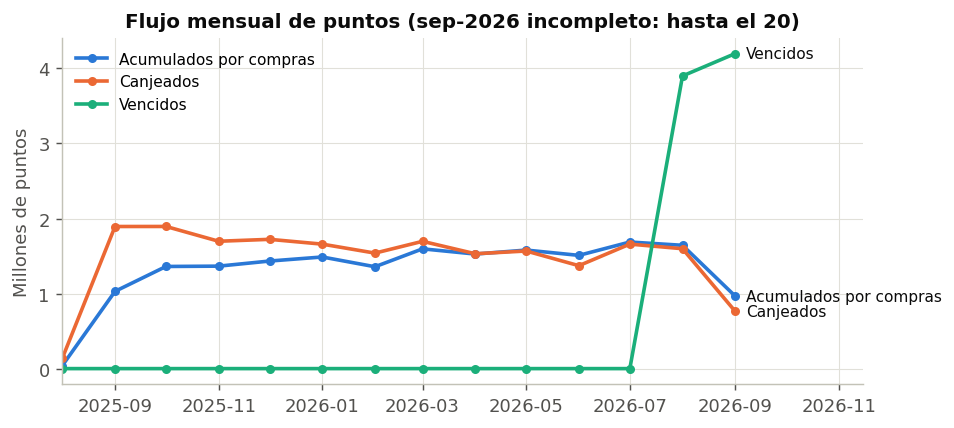
\includegraphics[width=0.85\textwidth]{imagenes/grafica_flujo_puntos.png}
\end{center}

\subsection{Otros hallazgos}

\begin{center}
\renewcommand{\arraystretch}{1.35}
\begin{tabular}{|>{\raggedright\arraybackslash}p{5.2cm}|>{\raggedright\arraybackslash}p{4cm}|>{\raggedright\arraybackslash}p{4.4cm}|}
\hline
\textbf{Hallazgo} & \textbf{Dato} & \textbf{Riesgo} \\
\hline
La app deja canjear en McDelivery sin llegar al mínimo (R15) & 33 canjes & La regla no está
implementada en la app \\
\hline
Terceros con pedidos grandes que el programa no ve & PedidosYa y Uber Eats: ticket de
$\sim$Q135 & Se desconoce a los clientes de mayor gasto \\
\hline
Cuentas de la misma persona & 150 cuentas & Abuso de la bienvenida \\
\hline
Saldos anteriores sin reclamar & 252 correos & Pasivo sin fecha clara \\
\hline
Eventos corruptos en la app & 55 sin cliente, restaurante o fecha & Compras que no acumulan y
generan reclamos \\
\hline
\end{tabular}
\end{center}

% ---------------------------------------------------
\section{6. Propuesta: un modelo de ML dentro del pipeline}

\subsection{Recomendador de recompensas}

La pregunta es qué recompensa mostrarle a cada cliente en la app, que es lo que McDonald's hace a
nivel corporativo con Dynamic Yield (Restaurant Technology News, 2026). El diseño es de
\textbf{dos etapas}, como los recomendadores reales: primero se toman como candidatas las
recompensas vigentes, y luego un modelo de \emph{gradient boosting} las ordena combinando el
gusto del cliente, el costo contra su saldo, la hora y la popularidad. El modelo queda registrado
en MLflow y en Unity Catalog, y escribe \texttt{gold\_recomendaciones} con un mensaje listo para la
app, por ejemplo: ``Te faltan 500 puntos para tu McFlurry''.

Tres decisiones de ingeniería que nos enseñaron algo:

\begin{itemize}[leftmargin=1.2em]
\item \textbf{Primero los baselines.} Con la primera versión de los datos, ningún modelo le ganaba
a ``recomendar lo más popular''. Faltaban gustos en los datos, así que generamos una segunda
versión con perfiles de gusto por cliente.
\item \textbf{Validación temporal.} Variables hasta el 20 de junio y etiqueta con los canjes del
20 de junio al 20 de septiembre: nada del futuro entra a las variables. Es la misma fuga de
información que vimos en el Ejercicio 1 con \texttt{score} y \texttt{winner}.
\item \textbf{El modelo evaluado es el que se despliega.} scikit-learn activa el
\emph{early stopping} solo cuando hay más de 10,000 filas, así que el modelo de producción se
estaba entrenando distinto al evaluado. Lo fijamos explícitamente.
\end{itemize}

\begin{center}
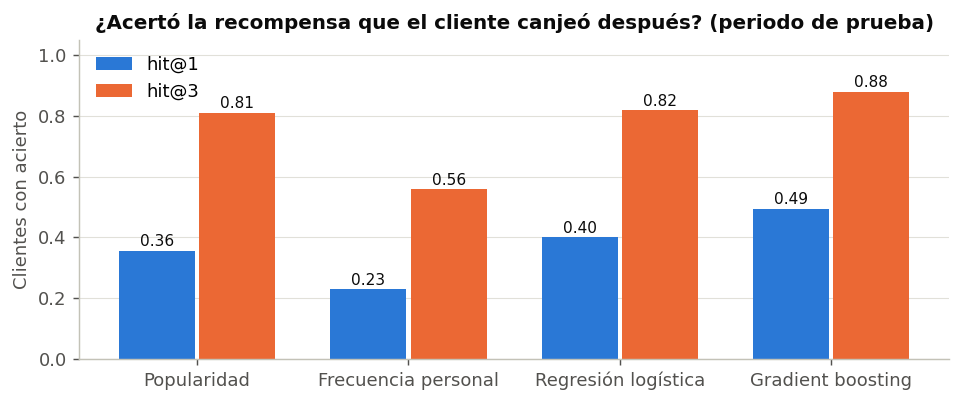
\includegraphics[width=0.85\textwidth]{imagenes/grafica_estrategias.png}
\end{center}

El modelo acierta la recompensa del banner principal (hit@1) un \textbf{39\,\% más} que
recomendar lo más popular (0.495 contra 0.356). Además revisamos si aprendió los gustos
\emph{reales}, que nunca vio:

\begin{center}
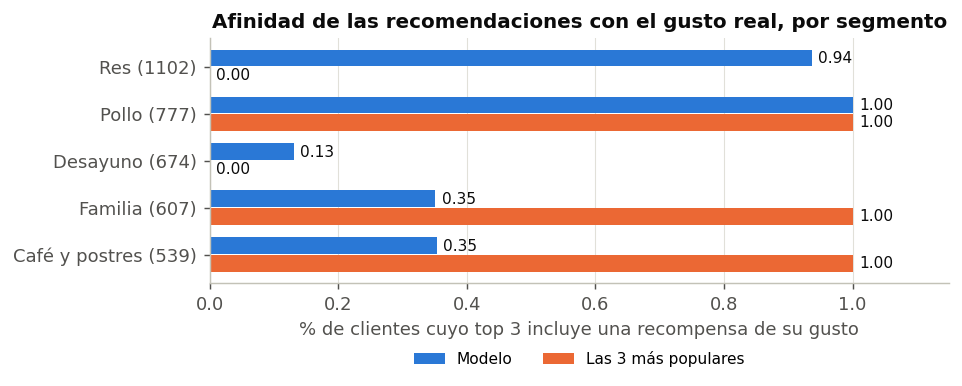
\includegraphics[width=0.85\textwidth]{imagenes/grafica_segmentos.png}
\end{center}

En total gana (0.62 contra 0.52), sobre todo en el segmento más grande (res). Pero lo que más nos
llamó la atención es el segmento desayuno: \textbf{ni el modelo ni la lista popular lo atienden}.
No es un problema del algoritmo sino del catálogo: las recompensas de desayuno cuestan 5,000 y
7,500 puntos, y la única barata, el café, salió en junio. También vimos que la variable que más
pesa es el costo: el modelo predice bien lo que la gente canjea, que es lo barato. Si McDonald's
quiere otro resultado, como más visitas o un ticket más alto, \textbf{el objetivo del modelo es
una decisión de negocio}, no técnica.

\subsection{Cómo se integra}

\begin{center}
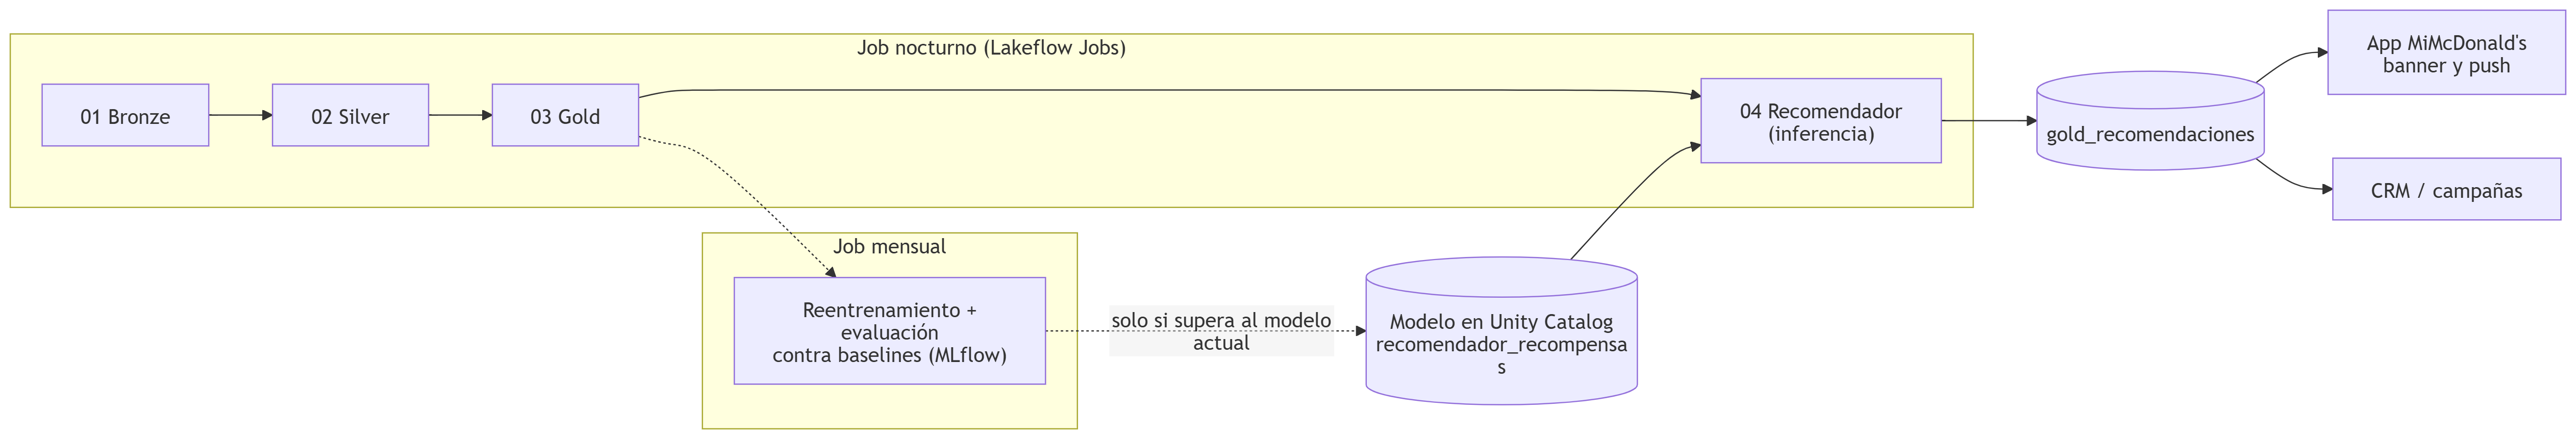
\includegraphics[width=\textwidth]{imagenes/integracion_ml.png}
\end{center}

\begin{center}
\renewcommand{\arraystretch}{1.35}
\begin{tabular}{|>{\raggedright\arraybackslash}p{3.4cm}|>{\raggedright\arraybackslash}p{10.2cm}|}
\hline
\textbf{Aspecto} & \textbf{Propuesta} \\
\hline
Inferencia & Nocturna, después de Gold, con el saldo del día \\
\hline
Reentrenamiento & Mensual o cuando cambie el catálogo; el modelo nuevo solo reemplaza al actual si
le gana a él y a los baselines \\
\hline
Monitoreo & hit@1 semanal con los canjes reales, clics del banner y diversidad de lo recomendado \\
\hline
Validación real & Prueba A/B: la mitad ve el catálogo actual y la otra mitad el recomendado,
durante 30 días \\
\hline
Extensión con LLM & Un LLM (\texttt{ai\_query()} en Databricks) redacta el mensaje, pero
\textbf{no} decide qué recompensa ofrecer \\
\hline
\end{tabular}
\end{center}

% ---------------------------------------------------
\section{7. Propuestas de optimización}

\begin{center}
\renewcommand{\arraystretch}{1.35}
\begin{tabular}{|p{1.4cm}|>{\raggedright\arraybackslash}p{5cm}|>{\raggedright\arraybackslash}p{7.2cm}|}
\hline
\textbf{Prioridad} & \textbf{Problema} & \textbf{Propuesta} \\
\hline
Alta & El tope diario castiga a McDelivery & Subir el tope o excluir a McDelivery; como mínimo,
avisarle al cliente en la app \\
\hline
Alta & La app no valida el mínimo de canje & Validar en la app y en el motor de lealtad, y
auditar con la tabla de violaciones \\
\hline
Alta & Cuentas duplicadas cobran la bienvenida & Verificar el teléfono al registrarse (OTP) \\
\hline
Media & Breakage alto & Avisar 30 días antes de vencer (R11), con una recompensa recomendada \\
\hline
Media & Segmentos sin recompensa accesible & Una recompensa de desayuno de unos 3,000 puntos y una
de Cajita Feliz \\
\hline
Media & Terceros invisibles para el programa & Integrar el código de lealtad en PedidosYa y Uber
Eats \\
\hline
Media & Reglas sin documentar & Adoptar nuestra documentación como oficial y validar H1--H8 con el
negocio \\
\hline
Técnica & Pipeline por lotes completos & Auto Loader para ingesta incremental, \texttt{MERGE} en
Gold, movimientos de reverso para anulaciones tardías, \emph{expectations} de Lakeflow y
orquestación con Lakeflow Jobs \\
\hline
\end{tabular}
\end{center}

% ---------------------------------------------------
\section{Conclusiones}

\begin{enumerate}[leftmargin=1.4em]
\item \textbf{El sistema se puede documentar y auditar desde afuera.} Reconstruimos 22 reglas con
fuentes públicas, encontramos 8 vacíos y los resolvimos con supuestos explícitos que el cliente
debe validar.

\item \textbf{La arquitectura medallion es la adecuada para un programa de puntos.} La acreditación
en 24 horas ya indica procesamiento por lotes, y separar la evidencia (Bronze), la limpieza
(Silver) y las reglas (Gold) permite auditar cualquier saldo y cambiar una regla sin tocar lo
demás.

\item \textbf{El diseño del modelo de datos pesa más que la herramienta.} Como los puntos vencen
por lote, el saldo no puede ser un número guardado: tiene que salir de un ledger.

\item \textbf{La réplica es confiable.} La POC pasó 39 de 39 pruebas: saldos idénticos en 5,150
clientes contra una implementación independiente y detección exacta de los 17 tipos de error.

\item \textbf{En nuestra opinión, lo más valioso del ML fue lo que reveló, más que lo que predijo.}
El recomendador le gana al baseline, pero dejó ver que el problema del segmento desayuno está en
el catálogo, y que qué optimizar es una decisión que le toca a McDonald's.

\item \textbf{Limitación:} los datos son sintéticos. La POC demuestra que el pipeline aplica bien
las reglas; el siguiente paso es validar esas reglas con el cliente y correr el pipeline con sus
datos reales.
\end{enumerate}

% ---------------------------------------------------
\section{Repositorio}

\url{https://github.com/DiegoLinares11/MLOPS-Caso-de-estudio-2}

Contiene la documentación de cada fase (\texttt{docs/}), los diagramas en Mermaid
(\texttt{diagramas/}), los seis notebooks de Databricks (\texttt{notebooks/}) y este reporte con
sus datos e imágenes (\texttt{reporte/}).

% ---------------------------------------------------
\section{Referencias}

\begin{referencias}

\item Chapman, P., Clinton, J., Kerber, R., Khabaza, T., Reinartz, T., Shearer, C., \& Wirth, R.
(2000). \emph{CRISP-DM 1.0: Step-by-step data mining guide}. SPSS.

\item Databricks. (s.f.). \emph{What is a medallion architecture?}
\url{https://www.databricks.com/glossary/medallion-architecture}

\item L'Express Franchise. (2026). \emph{McDonald's llega a 126 restaurantes en Guatemala: quién es
el dueño}.
\url{https://lexpress-franchise.com/latam/ultimas-noticias/mcdonalds-llega-126-restaurantes-guatemala-quien-es-dueno/}

\item McDonald's Corporation. (2023). \emph{McDonald's announces new targets for development,
loyalty membership, and cloud technology}.
\url{https://corporate.mcdonalds.com/corpmcd/our-stories/article/mcd-announces-targets-development-loyalty-membership-cloud-tech.html}

\item McDonald's Guatemala. (s.f.-a). \emph{Términos y Condiciones App de McDonald's en
Guatemala}. \url{https://mcdonaldsdigital.com/GML/public/app/gt/terminos-y-condiciones}

\item McDonald's Guatemala. (s.f.-b). \emph{MiMcDonald's Guatemala}.
\url{https://www.mi.mcdonalds.com.gt/}

\item McDonald's Guatemala. (s.f.-c). \emph{Puntos McDelivery}.
\url{https://puntosmcdelivery.mcdonalds.com.gt/}

\item Periódico Digital Centroamericano y del Caribe. (2025). \emph{McDonald's lanza
``MiMcDonald's'', su nuevo programa de lealtad para recompensar a sus invitados}.
\url{https://newsinamerica.com/pdcc/noticias/gerenciales/2025/mcdonalds-lanza-mimcdonalds-su-nuevo-programa-de-lealtad-para-recompensar-a-sus-invitados/}

\item Perspectiva. (2026). \emph{McDonald's alcanza 126 restaurantes en Guatemala}.
\url{https://perspectiva.gt/empresa/mcdonalds-alcanza-126-restaurantes-guatemala-2026/}

\item Restaurant Technology News. (2026). \emph{McDonald's unifies data from nearly 220 million
loyalty users as global AI strategy takes shape}.
\url{https://restauranttechnologynews.com/2026/08/mcdonalds-unifies-data-from-nearly-220-million-loyalty-users-as-global-ai-strategy-takes-shape/}

\end{referencias}

\end{document}
